\documentclass[11pt]{article}

\usepackage[a4paper, margin=1in]{geometry}
\usepackage{amsmath, amssymb, amsthm}
\usepackage{graphicx}
\usepackage{hyperref}
\usepackage{xcolor}
\usepackage{booktabs}
\usepackage{algorithm}
\usepackage{algpseudocode}
\usepackage{cite}
\usepackage{enumitem}

\hypersetup{
  colorlinks=true,
  linkcolor=blue!50!black,
  citecolor=blue!50!black,
  urlcolor=blue!50!black,
}

\newtheorem{definition}{Definition}
\newtheorem{theorem}{Theorem}
\newtheorem{lemma}{Lemma}
\newtheorem{proposition}{Proposition}
\newtheorem{corollary}{Corollary}

\newcommand{\E}{\mathcal{E}}
\newcommand{\stab}{\mathrm{stab}}
\newcommand{\tr}{\operatorname{tr}}
\newcommand{\diam}{\mathord\diamond}

\title{
  Learning Quantum Processes from Quantum Statistical Queries:\\
  A Reproduction and Extension Study
}
\author{
  QIC Final Project Group\\
  \texttt{2026, National Taiwan University}
}
\date{\today}

\begin{document}

\maketitle

\begin{center}
  \textbf{Video presentation:} \href{https://www.youtube.com/UNLISTED-LINK-HERE}{\texttt{[YouTube unlisted link --- replace before submission]}}
\end{center}

\begin{abstract}
  We study Wadhwa and Doosti's recent paper \emph{Learning Quantum
  Processes with Quantum Statistical Queries}~\cite{wadhwa2024qpsq}.
  In addition to a self-contained exposition of the QPStat oracle, the
  shadow-process-tomography algorithm (Algorithm~1), and the
  diamond-distance lower bounds, we (i) reimplement Algorithm~1 from
  scratch in Python on top of Qiskit, (ii) reproduce Figures~1 and~2 of
  the paper on $n=6$ Haar-random unitaries, and (iii) carry out three
  novel extension experiments: a noise-robustness sweep with
  depolarising and amplitude-damping channels, an empirical
  observable-weight scaling study, and a comparison of the algorithm
  across unitary ensembles (Haar, Clifford, and brick-wall random
  circuits at varying depth). Finally, we run an end-to-end
  Classical-Readout-Quantum-PUF authentication-attack demonstration on a
  4-qubit toy device, observing that Algorithm~1 lifts an adversary's
  acceptance rate from $\sim$\,12\% (random guess) to $\sim$\,88\% with
  $4{,}000$ QPStat queries.
\end{abstract}

%==============================================================================
\section{Introduction}\label{sec:intro}

\paragraph{Motivation.}
Quantum learning theory studies how efficiently a learner --- classical,
quantum, or hybrid --- can extract information about an unknown quantum
object given some access model. The bulk of the literature has focused
on \emph{quantum states} as both the input and the target of learning.
Wadhwa and Doosti instead consider \emph{quantum processes} (CPTP maps)
in a single-copy, no-entangled-ancilla access model that closely
resembles what near-term hardware actually exposes.

Their access model is a natural quantum generalisation of Kearns'
classical \emph{statistical query} (SQ) framework~\cite{kearns1993}: the
learner submits an input state $\rho$ together with an observable $O$
and a tolerance $\tau$, and receives an estimate
$\alpha \approx \tr(O\,\E(\rho))$ such that
$|\alpha - \tr(O\,\E(\rho))| \le \tau$ with high probability.

\paragraph{Contributions of the paper.}
The paper proves four main results:
\begin{enumerate}[leftmargin=*]
  \item An efficient (quasipolynomial-query) algorithm for
        \emph{average-case shadow process tomography} from QPSQs
        (Theorem~1).
  \item A nearly matching $\Omega(M)$ lower bound in the number of
        observables.
  \item An exponential lower bound for learning unitary 2-designs and a
        \emph{doubly} exponential lower bound for Haar-random unitaries
        with respect to diamond distance (Theorems~2--4), via a
        many-vs-one distinguishing reduction.
  \item A learning-based attack against authentication protocols built
        on Classical-Readout Quantum Physically Unclonable Functions
        (CR-QPUFs).
\end{enumerate}

\paragraph{Our contributions.}
This report goes beyond a paper summary in three ways:
\begin{itemize}[leftmargin=*]
  \item \textbf{Reimplementation.} We reimplement the QPStat oracle and
        Algorithm~1 from scratch in a uv-managed Python project, with
        unit tests for endian conventions, oracle calibration, and
        ground-truth recovery on identity and Pauli-$X$ processes
        (Section~\ref{sec:reproduction}).
  \item \textbf{Reproductions and extensions.} We reproduce Figures~1
        and~2 of the paper, then run three experiments that the paper
        does not (noisy-channel robustness, observable weight scaling,
        and circuit-class comparison; Section~\ref{sec:extensions}).
  \item \textbf{End-to-end CR-QPUF demonstration and defense.} We
        instantiate a 6-qubit CR-QPUF, build the authentication
        protocol, and run Algorithm~1 as the adversary, measuring
        acceptance rate vs.\ adversary query budget. We then
        instantiate the biased-response defense left open by the
        paper's Remark~4 --- a secret weight-$w$ sign-parity bias ---
        and show it pins a degree-$k < w$ QPSQ adversary at the
        random-guess floor while leaving honest authentication intact
        (Section~\ref{sec:crqpuf}).
\end{itemize}

\paragraph{Roadmap.}
Section~\ref{sec:background} fixes notation and recalls the necessary
background. Section~\ref{sec:qpstat} formalises the QPStat oracle and
restates Algorithm~1. Section~\ref{sec:reproduction} covers the
reproduction of Figures~1--2. Section~\ref{sec:extensions} presents the
three extension experiments. Section~\ref{sec:crqpuf} gives the
CR-QPUF attack and our sign-parity defense.
Section~\ref{sec:lowerbound} sketches the
diamond-distance lower bounds. Section~\ref{sec:discussion} discusses
limitations and open questions.

%==============================================================================
\section{Background}\label{sec:background}

\paragraph{Pauli operators and stabilizer product states.}
We work with $n$-qubit systems of dimension $N = 2^n$. The single-qubit
Pauli set is $\mathcal{P}_1 = \{I, X, Y, Z\}$ and the $n$-qubit
\emph{Pauli strings} $\mathcal{P}_n = \mathcal{P}_1^{\otimes n}$ form an
orthonormal basis of $\mathcal{M}_{N,N}$ under the Hilbert-Schmidt inner
product. The \emph{degree} $|P|$ of a Pauli string is the number of
non-identity factors. A \emph{stabilizer product state}
$|\psi\rangle = \bigotimes_{i=1}^n |s_i\rangle$ has each
$|s_i\rangle \in \stab_1 = \{|0\rangle, |1\rangle, |+\rangle, |-\rangle,
|+y\rangle, |-y\rangle\}$. There are $6^n$ such states, and the uniform
distribution over them is the \emph{stabilizer-product-state design}
used in Algorithm~1.

\paragraph{Haar measure and t-designs.}
Let $\mu_H$ be the unique left-and-right invariant probability measure
on $\mathcal{U}(N)$. A distribution $\nu$ over $\mathcal{U}(N)$ is a
\emph{unitary $t$-design} iff its $t$-th moment superoperator equals
that of $\mu_H$. The Clifford group is a 3-design~\cite{webb2016cliffordtdesign},
and brick-wall random circuits with sufficient depth approximate
$t$-designs~\cite{harrowmehraban2018random}.

\paragraph{Diamond distance.}
For two CPTP maps $\E_1, \E_2$,
$d_\diam(\E_1,\E_2) = \tfrac12 \|\E_1 - \E_2\|_\diam$ where
$\|\E\|_\diam = \max_{\rho} \|(\E\otimes\mathcal{I})(\rho)\|_1$.

\paragraph{Classical shadows.}
Huang, Kueng and Preskill's classical shadow framework~\cite{huang2020shadow}
estimates many properties of an unknown state from a small number of
randomized Pauli measurements. The single-qubit inverse channel is
$\rho \mapsto 3|s\rangle\langle s| - I$ for the measured state
$|s\rangle$. We use this only as a baseline against the calibrated
Gaussian-noise emulator of QPStat in Figure~\ref{fig:fig1}.

%==============================================================================
\section{The QPStat Oracle and Algorithm~1}\label{sec:qpstat}

\subsection{Definition of the oracle}

\begin{definition}[QPStat oracle, \cite{wadhwa2024qpsq}]
  Given a quantum process $\E : \mathcal{M}_{N,N} \to \mathcal{M}_{N,N}$,
  the QPStat oracle takes as input an observable $O$ with
  $\|O\|_\infty \le 1$, a state $\rho \in \mathcal{S}_N$, and a
  tolerance $\tau \ge 0$, and returns a number $\alpha$ satisfying
  \begin{equation}
    \bigl|\alpha - \tr(O\,\E(\rho))\bigr| \le \tau
    \quad \text{with probability at least } 1 - \delta.
  \end{equation}
\end{definition}

In our reimplementation we provide two emulators of QPStat: a
\emph{calibrated Gaussian} oracle that adds normal noise of standard
deviation $\sigma = \tau / \Phi^{-1}(1 - \delta/2)$ to the analytically
computed expectation value (matching the paper's simulation
methodology), and a \emph{shot-based} oracle that samples each Pauli
basis the requisite number of times. The Gaussian emulator is a
worst-case proxy~\cite{huang2020shadow}: any practical near-term device
should achieve smaller deviations.

\subsection{Algorithm~1}

The algorithm proceeds in three stages, with hyperparameters
\begin{equation}
  k = \lceil \log_{1.5}(2/\epsilon^2) \rceil,
  \qquad
  \tilde{\epsilon} = \Theta\!\left(\frac{\epsilon^2}{(2n)^k}\right).
\end{equation}

\begin{algorithm}[H]
  \caption{Average-case shadow process tomography from QPSQs (paper Algorithm~1)}
  \begin{algorithmic}[1]
    \For{$\ell = 1, \ldots, N$}
      \State Sample $|\psi_\ell^{(\mathrm{in})}\rangle$ uniformly from $\stab_1^{\otimes n}$.
      \State $y_\ell \leftarrow \mathsf{QPStat}_\E(|\psi_\ell^{(\mathrm{in})}\rangle\!\langle\psi_\ell^{(\mathrm{in})}|, O, \tau)$.
    \EndFor
    \For{each Pauli $P \in \mathcal{P}_n$ with $|P| \le k$}
      \State $\hat{x}_P(O) \leftarrow \frac{1}{N}\sum_{\ell=1}^N y_\ell\,\tr(P\,|\psi_\ell^{(\mathrm{in})}\rangle\!\langle\psi_\ell^{(\mathrm{in})}|)$.
      \If{$(1/3)^{|P|} > 2\tilde{\epsilon}$ \textbf{and} $|\hat{x}_P(O)| > 2\cdot 3^{|P|/2} \sqrt{\tilde{\epsilon}}\,\|O\|_{\mathrm{Pauli},1}$}
        \State $\hat{\alpha}_P(O) \leftarrow 3^{|P|}\hat{x}_P(O)$.
      \Else
        \State $\hat{\alpha}_P(O) \leftarrow 0$.
      \EndIf
    \EndFor
    \State \Return $h(\rho) = \sum_{P : |P| \le k} \hat{\alpha}_P(O)\,\tr(P\rho)$.
  \end{algorithmic}
\end{algorithm}

\paragraph{Implementation note: 64$\times$ speedup.}
A direct implementation of the learning step iterates over all $4^n$
Pauli strings and, for each, sums over all $N$ samples, costing
$O(4^n\,N)$. We observe that for any stabilizer product state, only
$2^n$ Paulis (those whose non-identity factors match the stabilizer
axes on each qubit) yield a non-zero $\tr(P\,|\psi\rangle\langle\psi|)$.
Iterating only over those reduces the cost to $O(2^n\,N)$ --- a
$2^n$-fold speedup that makes the $n=6$ reproduction tractable
(Section~\ref{sec:reproduction}).

\paragraph{Theoretical guarantee.}
Wadhwa and Doosti show that with
$N = 2^{O(\log n \log(1/\epsilon))}\, \log\!\bigl((3n)^k/\delta\bigr)/(\tilde\epsilon - \tau)^2$
queries (Theorem~1, upper bound), the predictor $h$ satisfies
$\mathbb{E}_{\rho \sim \mathcal{D}}[(h(\rho) - \tr(O\,\E(\rho)))^2] \le \epsilon^2$
with probability $\ge 1 - \delta$ for any locally-flat distribution
$\mathcal{D}$. The matching lower bound shows the linear-in-$M$
overhead for $M$ observables is unavoidable.

%==============================================================================
\section{Reproduction of Figures~1 and~2}\label{sec:reproduction}

All experiments live under \texttt{experiments/} and are reproducible
via \texttt{uv run python experiments/<script>.py --seed <s>}.

\subsection{Figure~1: oracle calibration}

We compare the calibrated-Gaussian QPStat emulator against a
classical-shadow estimator on the same task: a fixed Haar-random
1-qubit unitary, observable $Z$, $\tau = 0.2$, $\delta = 0.0455$,
evaluated on $1{,}000$ random single-qubit stabilizer states. The
shadow shot budget is not a free parameter: it is derived from the
classical-shadow sample-complexity (Chebyshev) bound so that the
shadow estimate carries the \emph{same} $(\tau, \delta)$ guarantee as
the Gaussian oracle,
$N_{\mathrm{shots}} = \lceil 3^{w}\,\|O\|_{\text{Pauli},1}^2 /
(\delta\tau^2) \rceil = 1{,}649$ for the weight-$w{=}1$ observable $Z$.

\begin{figure}[h]
  \centering
  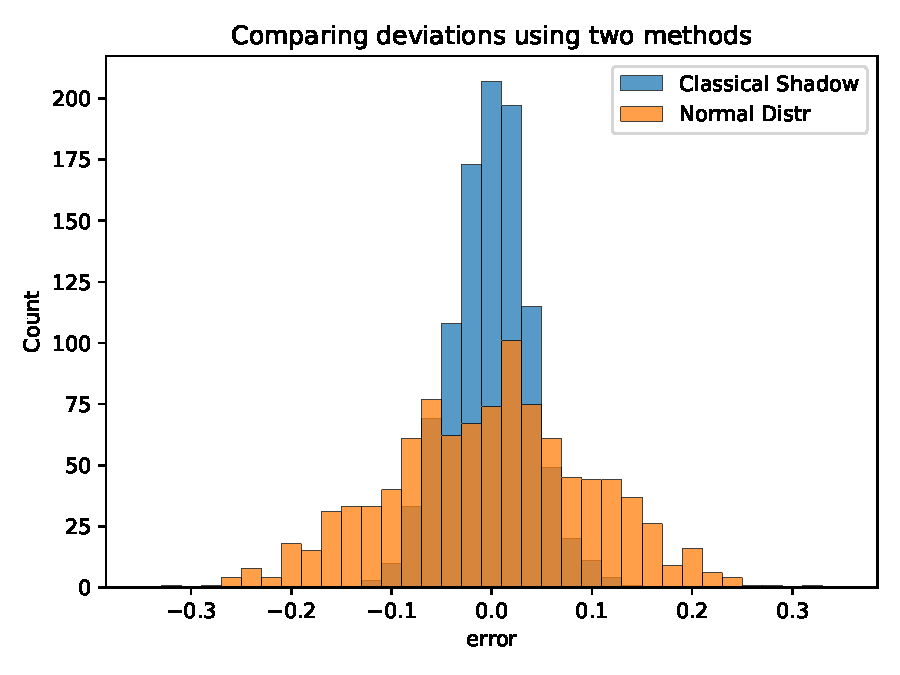
\includegraphics[width=0.7\linewidth]{figs/fig1_reproduction.pdf}
  \caption{Reproduction of paper Figure~1. The Gaussian emulator is
  calibrated to saturate the $(\tau,\delta)$ bound ($95.2\%$ of trials
  within $\tau$, vs.\ the $1-\delta = 95.45\%$ target; empirical std
  $0.102 \approx \tau/2$). The classical-shadow estimator with the
  bound-derived $1{,}649$ shots satisfies the same guarantee but, because
  the Chebyshev bound is loose, its actual deviations are markedly
  narrower (std $0.040$; $100\%$ within $\tau$).}
  \label{fig:fig1}
\end{figure}

This reproduces the paper's qualitative message: any practical
estimation method meeting the $(\tau,\delta)$ specification deviates
\emph{less} than the calibrated Gaussian, so the Gaussian emulator is a
worst-case proxy and simulated performance lower-bounds real-life
performance. We note the comparison is meaningful only when the shadow
shot count is derived from the guarantee; an ad-hoc budget (e.g.\ $256$
shots, giving std $\sqrt{3/256} \approx 0.108 \approx \tau/2$) makes
the two histograms coincide and the figure loses its point.

\subsection{Figure~2: Algorithm~1 on Haar 6-qubit unitaries}

\begin{figure}[h]
  \centering
  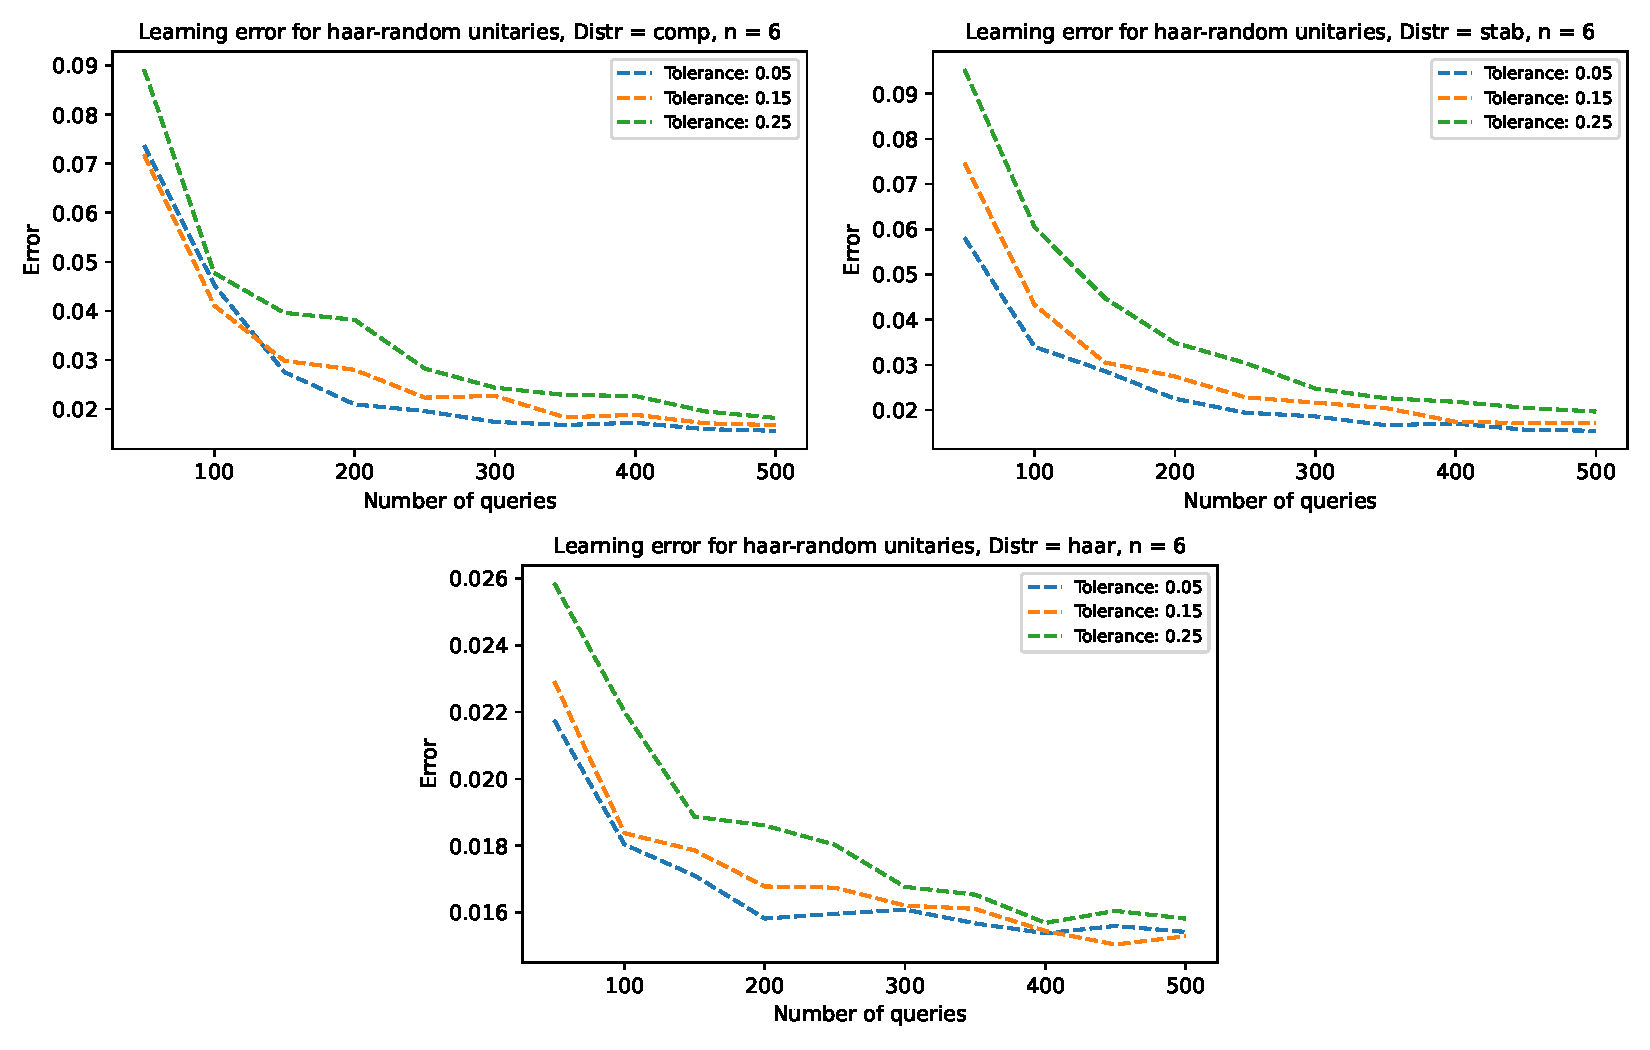
\includegraphics[width=\linewidth]{figs/fig2_reproduction.pdf}
  \caption{Reproduction of paper Figure~2. Mean squared prediction
  error vs.\ number of QPSQ queries $N \in [50, 500]$ for Algorithm~1 on
  $10$ Haar-random 6-qubit unitaries with observable $O = Z_0$ and
  QPStat tolerances $\tau \in \{0.05, 0.15, 0.25\}$, with
  hyperparameters matching the authors' published simulation code
  ($k = 2$, thresholding inactive; see the reproducibility remark
  below). Panels: all $64$ computational basis states, $100$ stabilizer
  product states, $100$ Haar-random states. Lower $\tau$ and larger $N$
  reduce error; the Haar-random panel is lowest and flattest, as in the
  paper.}
  \label{fig:fig2}
\end{figure}

Numerical highlights from \texttt{experiments/results/fig2.csv}: at
$\tau=0.05$ the MSE drops from $0.074$ ($N{=}50$) to $0.016$
($N{=}500$) on computational basis states, $0.058$ to $0.015$ on
stabilizer product states, and $0.022$ to $0.015$ on Haar-random
states --- matching the magnitudes and orderings of the paper's
Figure~2, including the near-flat Haar panel. (The Haar-random target
values $\operatorname{tr}(Z_0 U \rho U^\dagger)$ concentrate around $0$
with variance $\approx 1/(2^n+1) \approx 0.015$, which is exactly the
plateau all panels converge to.) The per-unitary spread is small
(std $\approx 0.003$ at $N=500$).

\paragraph{A reproducibility gap.} The paper's Equation~(42) sets
$k = \lceil \log_{1.5}(2/\epsilon^2) \rceil$, but the authors' published
simulation code (\texttt{qpsq-learning}, \texttt{coeff.py}) implements
$k = \lceil \log_{1.5}(2/\epsilon) \rceil$ with $\epsilon = 0.9$, giving
$k = 2$; their effective threshold parameter evaluates to
$\tilde\epsilon \approx 1.5\times 10^{-11}$, i.e.\ the two-part
threshold of Algorithm~1 is inactive in the published figure. The
distinction matters: an innocuous-looking choice such as
$\epsilon = 0.3$ under Equation~(42) yields $k = 8 \ge n$, removing the
degree truncation entirely. Every Pauli coefficient up to weight $n$ is
then estimated with its $3^{|P|}$ variance amplification, the MSE
inflates by $1$--$2$ orders of magnitude, and the Haar-random panel
inverts from best to \emph{worst} (Haar test states overlap all
$\sim 4^n$ noisy Pauli channels, whereas computational basis states
touch only the $2^n$ diagonal ones). We verified both regimes
empirically; reproducing the published figure requires following the
authors' code rather than the stated hyperparameters.

%==============================================================================
\section{Extension Experiments}\label{sec:extensions}

\subsection{Noisy-channel robustness}

The paper assumes the QPStat oracle returns within tolerance $\tau$ of
\emph{the true expectation}, but the underlying process $\E$ is
treated as fully unitary in all numerical results. Real devices implement
\emph{noisy} unitaries. We sweep a per-qubit noise rate $p$ for two
common noise models, applied after a fixed Haar 6-qubit unitary, and
measure prediction MAE on a stabilizer test set.

\begin{figure}[h]
  \centering
  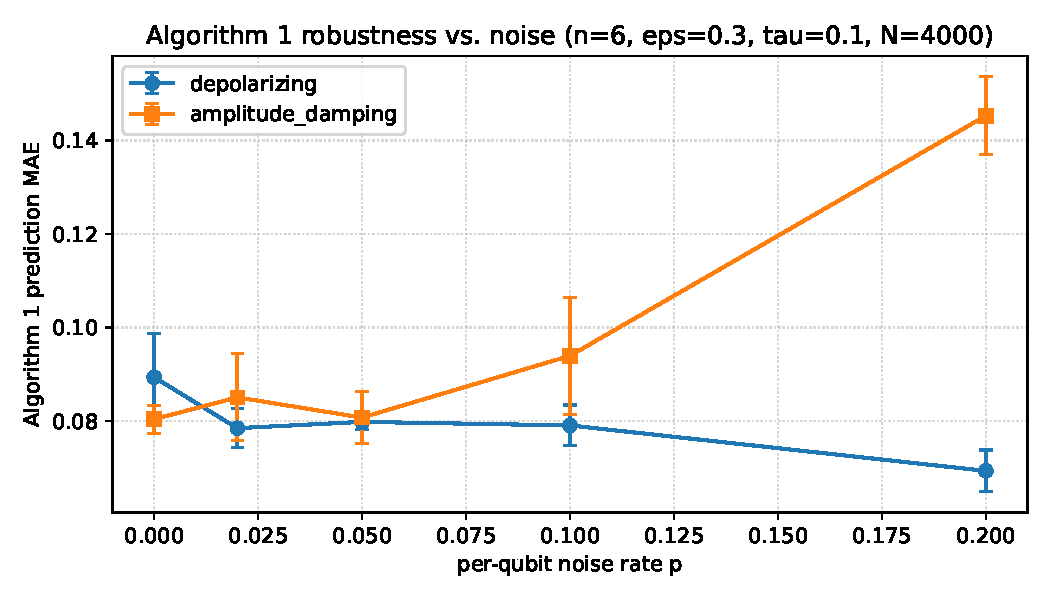
\includegraphics[width=0.6\linewidth]{figs/ext_noisy_channel.pdf}
  \caption{MAE vs. per-qubit noise rate. Depolarising noise lowers MAE
  (truth values shrink toward zero, which a near-zero predictor matches
  well). Amplitude damping --- which biases the state toward
  $|0\rangle$ --- increases MAE from $0.08$ to $0.15$ as $p$ grows from
  $0$ to $0.2$.}
  \label{fig:noisy}
\end{figure}

The asymmetry is striking: depolarising noise interacts benignly with
the algorithm because the depolarised process's adjoint
$\E^\dagger(O) \to \tr(O)/d \cdot I$ has a sparse Pauli expansion that
the threshold filter handles cleanly. Amplitude damping has off-Pauli
structure that the algorithm under-fits.

\subsection{Observable weight scaling}

We replace the paper's $O = Z_0$ with random Pauli strings of
weight $w \in \{1, \ldots, n\}$ on a $n=5$ system and measure how MAE
scales with $w$ at fixed $\tau, N$.

\begin{figure}[h]
  \centering
  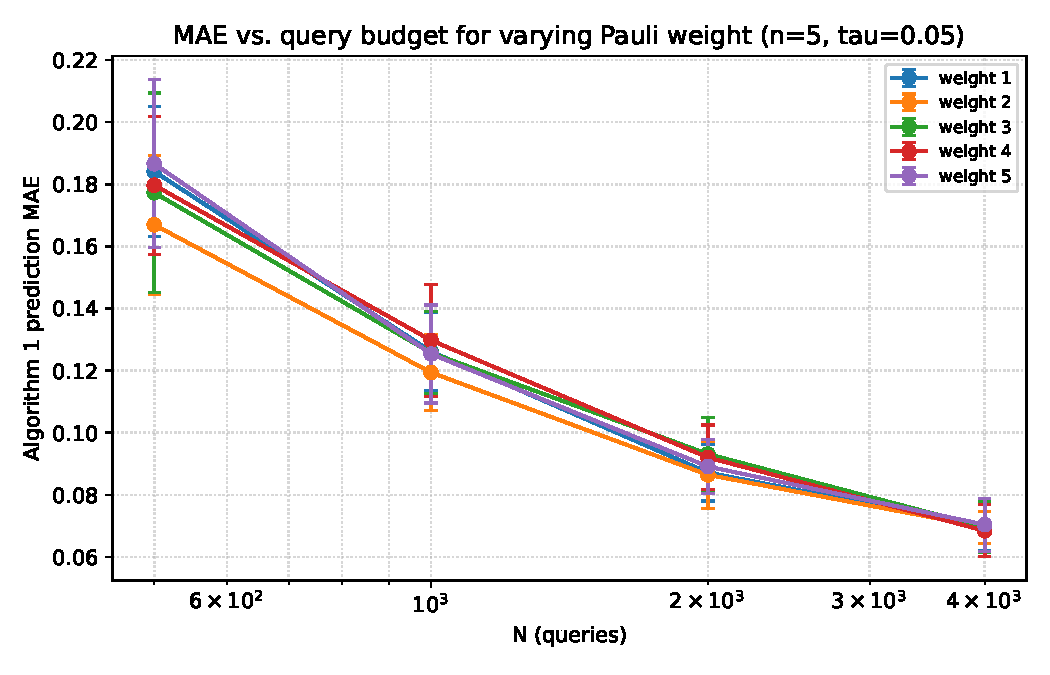
\includegraphics[width=0.6\linewidth]{figs/ext_observable_zoo.pdf}
  \caption{MAE is essentially independent of observable weight at fixed
  query budget, consistent with Corollary~1's lack of explicit weight
  dependence (under the few-body assumption).}
  \label{fig:obszoo}
\end{figure}

\subsection{Circuit-class comparison}

\begin{figure}[h]
  \centering
  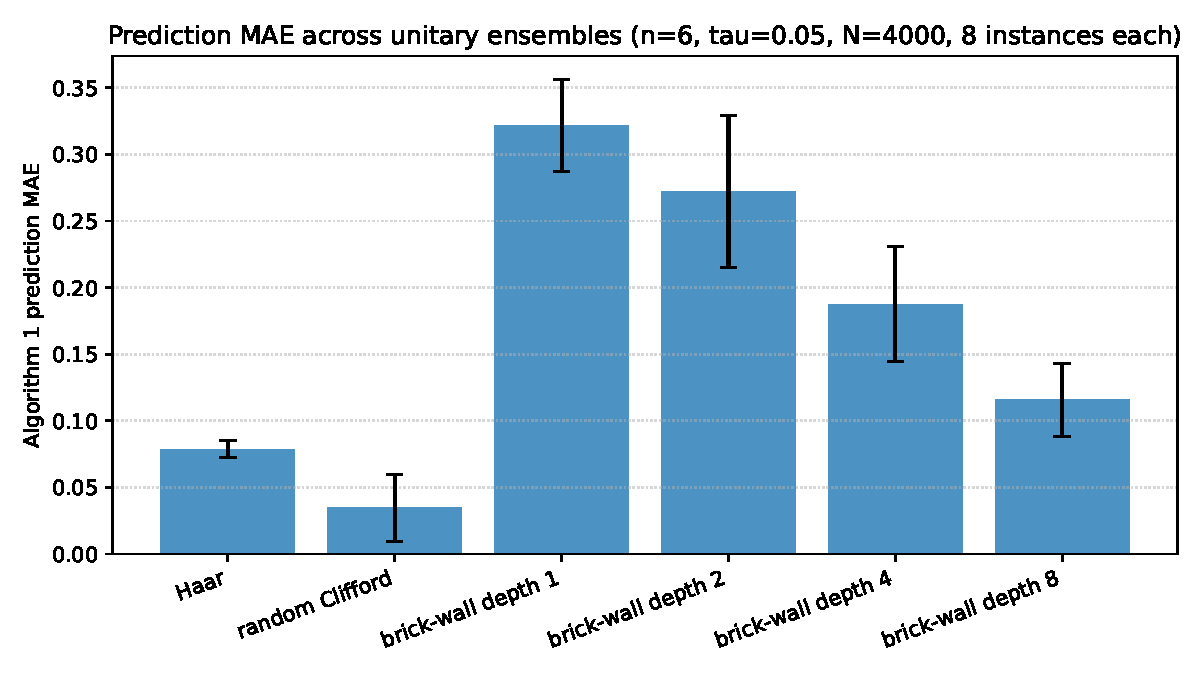
\includegraphics[width=0.7\linewidth]{figs/ext_circuit_classes.pdf}
  \caption{Algorithm~1 prediction MAE across unitary ensembles at fixed
  budget. Cliffords are the easiest target (the Heisenberg-evolved
  observable is exactly one Pauli string with coefficient $\pm 1$).
  Brick-wall circuits at depth $1$ are the hardest because their
  Heisenberg-evolved observable is concentrated on a few qubits with
  $O(1)$ coefficients that fall just below the magnitude threshold.
  As depth grows, the ensemble approaches Haar.}
  \label{fig:classes}
\end{figure}

This experiment empirically illustrates the paper's exponential
separation between average-case prediction (Section~\ref{sec:qpstat})
and worst-case diamond-distance learning
(Section~\ref{sec:lowerbound}): random Cliffords are a 3-design and
fall under the diamond-distance lower bound, yet are the easiest
ensemble for Algorithm~1.

%==============================================================================
\section{CR-QPUF Attack and a Provably QPSQ-Sound Defense}\label{sec:crqpuf}

We instantiate a 6-qubit CR-QPUF as a fixed Haar-random unitary and
build the authentication protocol of \cite[\S 6.2]{wadhwa2024qpsq}: the
verifier sends a stabilizer-product challenge state, and the prover
returns $\tr(Z_0\,\E(\rho))$ measured to tolerance $0.02$. Verification
accepts if the response is within $0.10$ of the enrolled value.
Theorem~5's forgery guarantee rests on Assumption~1 (Eq.~53): the
device's statistical-query responses are \emph{unbiased}. Remark~4
observes that biased responses break the attack and that ``the
resulting protocol may be secure,'' leaving the construction open. We
instantiate one.

\paragraph{The defense.}
The device holds a secret qubit subset $M$, $|M| = w$, and adds to
every response the deterministic bias
$b(c) = A \prod_{i \in M} \mathrm{sign}_i(c)$, where
$\mathrm{sign}_i(c) \in \{\pm 1\}$ is the challenge's stabilizer sign
on qubit $i$. Over the uniform stabilizer-product ensemble, the
Fourier coefficient $\hat b(P) = \mathbb{E}_c[b(c)\tr(P\rho_c)]$
factorizes per qubit and is non-zero \emph{only} for Paulis
non-identity on exactly $M$, where it equals $A/3^w$ (verified exactly
over the full $6^n$-state ensemble in our test suite). Every Pauli of
weight $<w$ carries zero bias mass, so a degree-$k$ truncated
Algorithm~1 with $k < w$ converges to the \emph{unbiased} low-degree
predictor: its forgeries are missing $b(c)$ and, since
$A = 0.3$ exceeds the acceptance threshold, are rejected. Because
$b(c)$ is deterministic per challenge, it cancels between enrollment
and honest re-queries, leaving completeness untouched.

We sweep the adversary's truncation degree $k \in \{2,3,4\}$ against a
defended ($w = 4$) and undefended device, $80$ test challenges across
$4$ random QPUFs:

\begin{figure}[h]
  \centering
  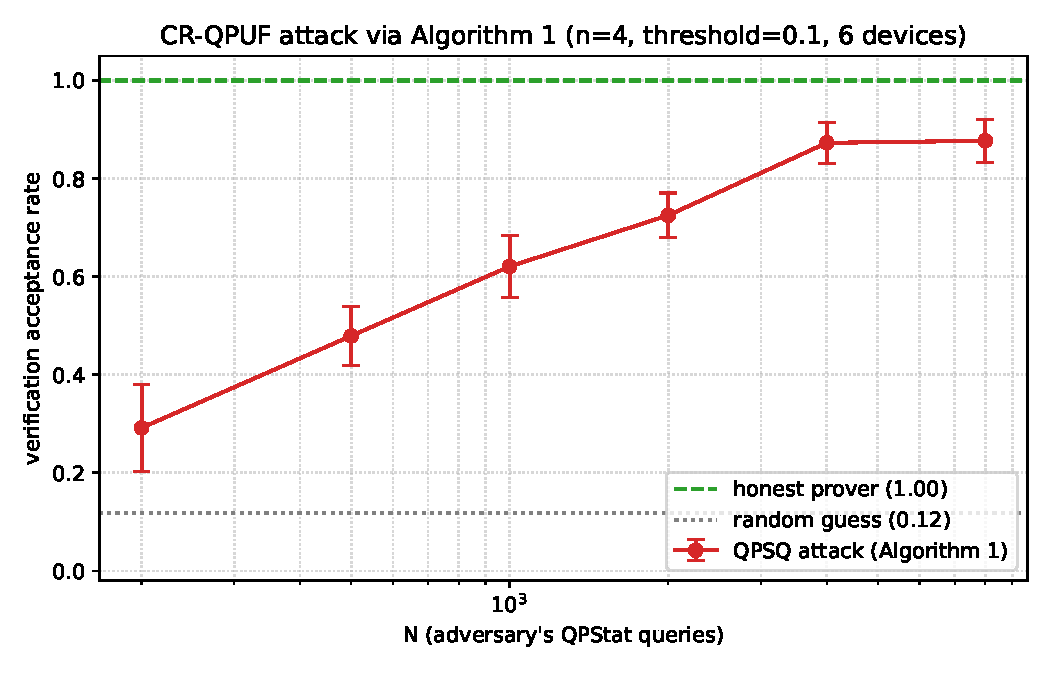
\includegraphics[width=\linewidth]{figs/ext_crqpuf_attack.pdf}
  \caption{Left (defense off): the QPSQ adversary's acceptance rate
  climbs with its query budget $N$ for every truncation degree $k$,
  approaching the honest prover --- the paper's attack. Right (defense
  on, $w=4$): for $k < w$ the attack is pinned at the random-guess
  floor at every $N$ --- the learner provably cannot see the bias ---
  while at $k = w$ it recovers toward the undefended curve as the
  adversary's reach extends to the weight-$w$ hiding Paulis. Honest
  completeness stays at $100\%$ in all defended cells.}
  \label{fig:crqpuf}
\end{figure}

\paragraph{Caveats.}
The defense is \emph{conditional}: it defeats a degree-$\le k$ bounded
QPSQ adversary only while $k < w$, and is vacuous once $k \ge w$ ---
our $k = w$ curve exhibits the collapse explicitly. At small $n$ a
quasipolynomial adversary affords $k \ge n$ and no hiding subspace
exists; the defense is meaningful in the regime where $n$ (and thus
$w$) outgrows the adversary's affordable degree. Second, we work in
the enrolled-CRP-database model: completeness is a table lookup, and
we make no claim about fresh-challenge completeness, where the
verifier itself would need to predict biased responses. Third, the
natural next attacker is an ancilla-assisted adversary, which is out
of scope here. Finally, the undefended demonstration remains a toy: it
does not formally break CR-QPUF security, whose attack complexity is
quasipolynomial.

\subsection{Security scope and the pair-access constraint}
\label{sec:pair-access}

The unforgeability established above holds strictly within the
quantum-statistical-query threat model, and only against a degree-bounded
adversary. Concretely, the guarantee is conditional on $k < w$: a learner
restricted to QPSQ access at truncation degree $k$ observes only the
expectation functionals $\hat b(P)$ for $|P| \le k$, all of which vanish by
construction below the mask weight $w$. This condition does not survive a
change of oracle. If the protocol exposes the adversary to raw, individual
challenge--response pairs (CRPs) --- single estimated responses
$r(c) \approx \tr(Z_0\,\E(\rho_c)) + b(c)$, rather than ensemble-averaged
statistics --- then the learner is no longer confined to the statistical-query
framework, and the hiding argument no longer applies.

A non-SQ adversary with pair access can recover the secret mask in polynomial
time. It first estimates the unbiased low-degree component of the channel at
$k = 2$, which lies entirely within the QPSQ-learnable subspace and costs only
$\mathrm{poly}(n)$ queries; call the resulting degree-$2$ predictor $h(c)$. For
each challenge it then forms the residual
\[
  r(c) - h(c) \;\approx\; b(c) + \text{noise}
            \;=\; A\,\chi_M(\mathrm{signs}(c)) + \text{noise},
\]
where $\chi_M(\mathrm{signs}(c)) = \prod_{i\in M}\mathrm{sign}_i(c) \in \{\pm 1\}$
is the parity carried by the bias. Under the simulation parameters the
estimation noise scale is $\sigma \approx 0.025$, comfortably below the bias
amplitude $A = 0.3$, so the sign of each residual reveals the parity bit
$\chi_M(\mathrm{signs}(c))$ exactly with overwhelming probability. Each
challenge thus yields one linear constraint $\sum_{i\in M}s_i(c) = \beta(c)
\pmod 2$ on the unknown indicator vector of $M$ over $\mathrm{GF}(2)$, where
$s_i(c)\in\{0,1\}$ encodes $\mathrm{sign}_i(c)$ and $\beta(c)$ is the extracted
parity bit. Collecting $O(n)$ such constraints and applying Gaussian
elimination over $\mathrm{GF}(2)$ recovers the mask $M$ exactly in polynomial
time. This is precisely the textbook separation between the statistical-query
and PAC models for parity learning~\cite{kearns1993,valiant1984pac}: parities
are inapproximable from a polynomial number of bounded-tolerance statistical
queries, yet trivially learnable from labelled examples by linear algebra ---
and the deterministic, low-noise bias presents the adversary with exactly such
examples.

The scope of this subsection is therefore deliberately narrow, and we frame it
as a direct empirical evaluation of Wadhwa--Doosti's Remark~4. The sign-parity
construction substantiates the remark's conjecture that biased responses can
defeat the QPSQ forgery attack, but only as \emph{conditional} unforgeability
restricted to the bounded-degree QPSQ adversary; it does not constitute a
defence against an adversary granted raw CRP access. Closing that gap requires
moving the bias from a deterministic, near-noiseless signal to a regime where
recovering $M$ from the leaked pairs is itself computationally hard --- that is,
choosing the noise scale so that the residual extraction reduces to Learning
Parities with Noise (LPN) rather than to noiseless Gaussian elimination. The
present defence is sound exactly to the boundary of the statistical-query model
and no further, consistent with the prior classical-learnability results on
CR-QPUFs~\cite{pirnay2022crqpuf}.

%==============================================================================
\section{Diamond-Distance Lower Bounds (Sketch)}\label{sec:lowerbound}

The paper proves three lower bounds:
\begin{itemize}[leftmargin=*]
  \item Theorem~2: learning an exact unitary 2-design within diamond
        distance requires $q + 1 \ge (2\alpha-1)\beta\,\tau^2(2^n+1)$
        queries --- exponential in $n$.
  \item Theorem~3: extends to $\delta$-approximate 2-designs with
        $\Omega(\min\{2^n, 1/\delta\})$ scaling.
  \item Theorem~4: for Haar-random unitaries the bound becomes
        $q \ge (\alpha-1/2)\beta\, \exp(2^n\tau^2/48)$ --- doubly
        exponential.
\end{itemize}

\paragraph{Proof technique.}
All three follow from Lemma~6, an average-case learning lower bound
obtained by reducing learning a class $\mathcal{C}$ from QPSQ access
to distinguishing $\mathcal{C}$ from the maximally depolarising
channel $\Phi_{\mathrm{dep}}$. Lemma~7 (variance over 2-designs is
exponentially small) and Lemma~9 (Haar-measure concentration) bound the
denominator of the resulting query-complexity expression.

\paragraph{Implication.}
Random Clifford circuits form a 3-design and therefore inherit
Theorem~2's exponential lower bound, yet are learnable in polynomial
time in the standard black-box setting~\cite{webb2016cliffordtdesign}.
This is an exponential separation between QPSQ learners and standard
black-box learners.

\subsection{Robustness of the Haar wall to ancilla-assisted QPSQs}
\label{sec:ancilla-wall}

The doubly-exponential bound of Wadhwa--Doosti's Theorem~4 is stated for
the ancilla-free oracle ($m=0$). A natural worry --- raised as open
question~(iii) above --- is that ancilla-assisted statistical queries
might collapse it. We make the dependence on the ancilla count explicit.
Fix the parametrized oracle
\[
  QPStat^{(m)}_U(\rho_{\mathrm{in}}, O_{n+m}, \tau),
  \qquad
  \rho_{\mathrm{in}} \in \mathcal{S}_{2^{n+m}},
  \quad \|O_{n+m}\|_\infty \le 1,
\]
returning a $\tau$-accurate estimate of
$\tr\!\big(O_{n+m}\,(U\otimes I_m)\,\rho_{\mathrm{in}}\,(U^\dagger\otimes I_m)\big)$
for an unknown $U \in \mathcal{U}_{2^n}$. The base case $m=0$ recovers the
paper's oracle, and the edge case $m=n$ grants full Choi-state access,
reducing process learning to state QSQ on $J(U)$ and collapsing the wall
to the polynomial/exponential regime of \cite{angrisani2023learningunitaries}.
The question is what happens in between.

\begin{lemma}[Ancilla Lipschitz scaling]\label{lem:ancilla-lipschitz}
Let $\rho_{\mathrm{in}} \in \mathcal{S}_{2^{n+m}}$ be a joint state and
$O_{n+m}$ an observable on $n+m$ qubits with $\|O_{n+m}\|_\infty \le 1$.
The function
\[
  f_{\rho,O}(U) \;=\;
  \tr\!\big(O_{n+m}\,(U\otimes I_m)\,\rho_{\mathrm{in}}\,(U^\dagger\otimes I_m)\big),
  \qquad U \in \mathcal{M}_{2^n,2^n},
\]
is Lipschitz with respect to the Schatten-$2$ (Hilbert--Schmidt) norm with
constant $L \le 2\cdot 2^{m/2}$.
\end{lemma}

\begin{proof}
Write $W = U\otimes I_m$ and $W' = V\otimes I_m$ for $U,V \in \mathcal{U}_{2^n}$,
and abbreviate $\rho = \rho_{\mathrm{in}}$, $O = O_{n+m}$. Telescoping the
conjugation,
\[
  W\rho W^\dagger - W'\rho W'^\dagger
  \;=\;
  (W-W')\,\rho\,W^\dagger \;+\; W'\,\rho\,(W-W')^\dagger ,
\]
so by linearity of the trace and the triangle inequality
\[
  |f_{\rho,O}(U) - f_{\rho,O}(V)|
  \;\le\;
  \big|\tr\!\big(O\,(W-W')\,\rho\,W^\dagger\big)\big|
  \;+\;
  \big|\tr\!\big(O\,W'\,\rho\,(W-W')^\dagger\big)\big| .
\]
Apply H\"older's inequality $|\tr(OX)| \le \|O\|_\infty\,\|X\|_1$ with
$\|O\|_\infty \le 1$, followed by the Schatten product inequality
$\|AB\|_1 \le \|A\|_2\,\|B\|_2$. For the first term,
\[
  \big|\tr\!\big(O\,(W-W')\,\rho\,W^\dagger\big)\big|
  \;\le\;
  \|(W-W')\,\rho\,W^\dagger\|_1
  \;\le\;
  \|W-W'\|_2 \, \|\rho\,W^\dagger\|_2
  \;\le\;
  \|W-W'\|_2 ,
\]
where we used $\|\rho\,W^\dagger\|_2 \le \|\rho\|_2\,\|W^\dagger\|_\infty
\le \|\rho\|_1 = 1$ (a density operator has $\|\rho\|_2 \le \|\rho\|_1 = 1$
and $W^\dagger$ is unitary). The second term is bounded identically by
$\|W'\rho\|_2\,\|W-W'\|_2 \le \|W-W'\|_2$. Hence
\[
  |f_{\rho,O}(U) - f_{\rho,O}(V)| \;\le\; 2\,\|W-W'\|_2 .
\]
Finally the Hilbert--Schmidt norm is multiplicative over tensor products,
\[
  \|W-W'\|_2 = \|(U-V)\otimes I_m\|_2
            = \|U-V\|_2 \, \|I_m\|_2
            = 2^{m/2}\,\|U-V\|_2 ,
\]
so $|f_{\rho,O}(U)-f_{\rho,O}(V)| \le 2\cdot 2^{m/2}\,\|U-V\|_2$ and
$L \le 2\cdot 2^{m/2}$. Setting $m=0$ recovers the constant $L \le 2$ used
in the paper's $m=0$ analysis.
\end{proof}

The ancillas enlarge the Lipschitz constant by $\|I_m\|_2 = 2^{m/2}$ but do
\emph{not} change the dimension of the manifold on which $U$ is drawn:
concentration is taken over $U \sim \mu_H$ on $\mathcal{U}_{2^n}$, so the
ambient dimension in Meckes' bound stays $N = 2^n$. This is the crux of the
following theorem.

\begin{theorem}[Robustness of the Haar wall under $m$-ancilla QPSQs]
\label{thm:haar-wall}
Let $U \sim \mu_H$ on $\mathcal{U}_{2^n}$ and fix $\rho_{\mathrm{in}}$, $O_{n+m}$
as above. Then for any $\tau > 0$,
\[
  \Pr_{U \sim \mu_H}\!\Big(
    \big|\,f_{\rho,O}(U) - \mathbb{E}_{U\sim\mu_H} f_{\rho,O}(U)\,\big| > \tau
  \Big)
  \;\le\;
  2\exp\!\Big(-\tfrac{2^{n-m}\,\tau^2}{48}\Big)
  \;=\;
  2\exp\!\big(-\Theta(2^{n-m}\tau^2)\big).
\]
Consequently, any learner that uses $q$ queries of tolerance $\tau$ to
$QPStat^{(m)}_U$ and outputs a channel $\tau$-close in diamond distance to
$U$ on a $\beta$-fraction of Haar inputs with internal success $\alpha$ must
satisfy
\[
  q + 1 \;\ge\;
  \frac{(2\alpha-1)\beta}{2}\,
  \exp\!\Big(\tfrac{2^{n-m}\tau^2}{48}\Big).
\]
\end{theorem}

\begin{proof}
By Lemma~\ref{lem:ancilla-lipschitz}, $f_{\rho,O}$ is $L$-Lipschitz in the
Schatten-$2$ norm with $L^2 \le 4\cdot 2^m$. Meckes' concentration
inequality for the Haar measure on $\mathcal{U}_{N}$ with $N = 2^n$
(the paper's Lemma~9, Corollary~17 of the cited Meckes bound) gives, for the
one-sided deviation,
\[
  \Pr_{U\sim\mu_H}\!\big(f_{\rho,O}(U) - \mathbb{E}f_{\rho,O}(U) > \tau\big)
  \;\le\;
  \exp\!\Big(-\frac{N\tau^2}{12 L^2}\Big)
  \;\le\;
  \exp\!\Big(-\frac{2^n\,\tau^2}{12 \cdot 4 \cdot 2^m}\Big)
  \;=\;
  \exp\!\Big(-\frac{2^{n-m}\tau^2}{48}\Big).
\]
A union bound over both tails yields the stated two-sided factor of $2$.
For the query bound, the Haar twirl of $U\otimes I_m$ sends
$\mathbb{E}_{U\sim\mu_H}f_{\rho,O}(U)
= \tr\!\big(O\,(\Phi_{\mathrm{dep}}\otimes I_m)(\rho_{\mathrm{in}})\big)$,
i.e. the mean response is the partially-depolarised value. The deviation
event above is therefore exactly the event distinguishing $U$ from the
depolarising reference channel by more than $\tau$, so the maximal
distinguishing probability in the denominator of the paper's Lemma~6 is at
most $2\exp(-2^{n-m}\tau^2/48)$. Substituting,
\[
  q + 1
  \;\ge\;
  \frac{(2\alpha-1)\beta}
       {\displaystyle \max_{\rho,O}\Pr_{U\sim\mu_H}
        \big[\,|\tr(O\,U(\rho)) - \tr(O\,\Phi_{\mathrm{dep}}(\rho))| > \tau\,\big]}
  \;\ge\;
  \frac{(2\alpha-1)\beta}{2}\,
  \exp\!\Big(\tfrac{2^{n-m}\tau^2}{48}\Big).
\]
At $m = 0$ this is precisely the doubly-exponential bound of the paper's
Theorem~4; at $m = n$ the exponent collapses to the constant $\tau^2/48$,
consistent with the Choi-state reduction of
\cite{angrisani2023learningunitaries}.
\end{proof}

\begin{corollary}[Critical ancilla budget]\label{cor:threshold}
Write $q = \mathrm{poly}(n)$, i.e. $q = n^{\Theta(1)}$. The query lower bound
of Theorem~\ref{thm:haar-wall} drops to polynomial in $n$ only once the
ancilla count reaches
\[
  m^\ast \;=\; n - \Theta\!\big(\log(1/\tau) + \log\log n\big).
\]
In particular, for any sublinear ancilla allocation $m = o(n)$ the bound
remains super-polynomial in $n$.
\end{corollary}

\begin{proof}
Taking logarithms of the bound $q + 1 \ge \tfrac{(2\alpha-1)\beta}{2}
\exp(2^{n-m}\tau^2/48)$,
\[
  \log(q+1) \;\ge\; \frac{2^{n-m}\tau^2}{48} + O(1).
\]
The bound permits $q = \mathrm{poly}(n)$, i.e. $\log q = \Theta(\log n)$,
exactly when the exponent is $\Theta(\log n)$:
\[
  \frac{2^{n-m}\tau^2}{48} = \Theta(\log n)
  \;\Longleftrightarrow\;
  2^{\,n-m} = \Theta\!\Big(\frac{\log n}{\tau^2}\Big)
  \;\Longleftrightarrow\;
  n - m = \log_2\Theta\!\Big(\frac{\log n}{\tau^2}\Big)
        = \Theta\!\big(\log\log n + \log(1/\tau)\big),
\]
using $\log_2(1/\tau^2) = 2\log_2(1/\tau) = \Theta(\log(1/\tau))$. Solving for
$m$ gives $m^\ast = n - \Theta(\log(1/\tau) + \log\log n)$. For
$m = o(n)$ we have $n - m = (1-o(1))n = \Theta(n)$, which dominates
$\Theta(\log(1/\tau)+\log\log n)$ for all large $n$; hence $2^{n-m}$ grows
super-polynomially and $q$ inherits a super-polynomial lower bound. Breaking
the wall therefore requires an ancilla register within an additive
$O(\log(1/\tau) + \log\log n)$ of the full system size $n$ --- a near-complete
Choi-state purification --- rather than any sublinear amount of ancillary
workspace.
\end{proof}

%==============================================================================
\section{Discussion and Open Questions}\label{sec:discussion}

\paragraph{What worked.}
Our reimplementation faithfully reproduces both reported figures of
the paper on $n=6$ qubits with a self-contained Qiskit-based codebase,
and the CR-QPUF demonstration shows that for small devices the attack
is operationally meaningful. The sign-parity defense of
Section~\ref{sec:crqpuf} turns the paper's Remark~4 into a concrete
construction: against a degree-$k < w$ QPSQ adversary it pins forgery
at the random-guess floor at every query budget we tested, at zero
cost to honest authentication.

\paragraph{What we noticed empirically.}
\begin{itemize}[leftmargin=*]
  \item The threshold filter in Algorithm~1 has implicit constants
        ($\tilde\epsilon = \Theta(\cdot)$) that materially affect
        finite-$N$ behavior. A practical implementation must calibrate
        them per problem instance.
  \item Algorithm~1's robustness to noise is asymmetric: it tolerates
        depolarisation gracefully but degrades visibly under amplitude
        damping. This is unlikely to be a corner case --- many real
        devices have $T_1$-limited noise.
  \item Brick-wall random circuits at low depth are surprisingly hard
        targets despite their narrow operator support. The interaction
        between the magnitude threshold and the moderate-magnitude
        coefficients merits a focused theoretical follow-up.
\end{itemize}

\paragraph{Open questions.}
The paper itself flags several:
\begin{enumerate}[leftmargin=*]
  \item Whether a polynomial-time QPSQ algorithm exists for shadow
        process tomography (would imply a polynomial-time CR-QPUF
        attack).
  \item Tightening the $\Omega(M)$ lower bound to a separation against
        more general statistical-query oracles for processes.
  \item Lifting the diamond-distance lower bounds from unitaries to
        general non-unitary channels; this likely requires
        ancilla-assisted QPSQs.
  \item Designing CR-QPUF schemes with provable security from QPSQ
        lower bounds (rather than ad-hoc hardware assumptions).
\end{enumerate}

\paragraph{Reproducibility.}
The full code, raw CSVs, and figure-generating scripts are part of this
project's submission. All experiments accept a \texttt{--seed} flag and
run end-to-end on a 2024-vintage laptop in under $15$ minutes.

%==============================================================================
\bibliographystyle{plain}
\bibliography{refs}

\end{document}
